\chapter{Introduction}
\label{chap1}
Signals are time-varying quantities which carry information. They may be, for example, audio signals (speech, music), images or video signals, sonar signals or ultrasound, biological signals such as the electrical pulses from the heart, communications signals, or many other types. With the emergence of high-speed, low-cost computing hardware, we now have the opportunity to analyze and process signals via computer algorithms.\\

The basic idea is straightforward: Rather than design complex circuits to process signals, the signal is first converted into a sequence of numbers and processed via software. By its very nature, software is more easily extensible and more versatile as compared with hard-wired circuits, which are difficult to change. Furthermore, using software, we can build in more �intelligence� into the operation of our designs and thus develop more human-usable devices.
\section{Objectives}
%
%
The objectives of this project are:
%
%for 1,2,3 numbers
\begin{enumerate}
\item To get familiar with how to describe signals mathematically and understand how to perform mathematical
operations on signals.
%
\item It will provide knowledge of digital filter
%
\item To discuss word length issues ,multi rate signal processing and application.
%
%
\end{enumerate}
\section{Introduction}
\noindent Audio signal processing is the subfield of signal processing in which we work with the
audio or what we hear. Different objects produce sound like bird, engines, motors noise
in robotic systems. The human can hear these sounds but there is always a mixture of
some background noise in the audio signals that must be processed in order to
get the desire signals.
\begin{figure}[H]  %h=positioning
\begin{center}
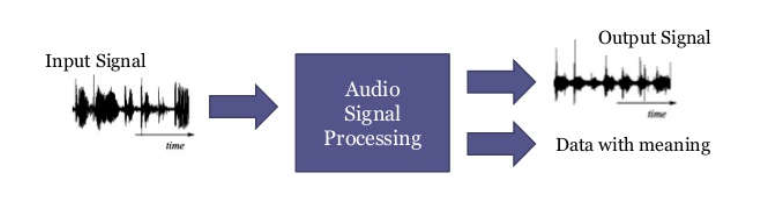
\includegraphics[scale=0.60]{Chapter1/figure1}
\caption{Audio Signal Processing}
\label{figure1}
\end{center}
\end{figure}

The audio sample is taken having some background noise or by adding noise by yourself,
then this audio sample is processed by analyzing it in MATLAB or any other tools. We
perform some operation of the signal, for more precisely analyzing the signals in
Frequency spectrum for analyzing in frequency domain in order to remove noise. Then a
filtered signal is produced at the output.
\begin{figure}[H]  %h=positioning
\begin{center}
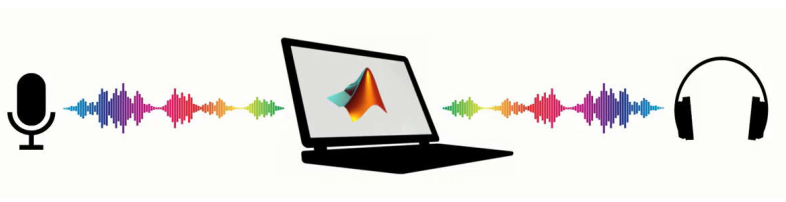
\includegraphics[scale=0.60]{Chapter1/figure2}
\caption{Signal Processing Technique}
\label{figure2}
\end{center}
\end{figure}

\subsection{Filters}
\subsubsection{Bandpass Filters}
A bandpass filter is an filter that allows signals between two explicit frequencies,
however that oppresses signals at different frequencies. Some bandpass channels
require an outer wellspring of intensity and utilize dynamic parts, for example,
semiconductors and coordinated circuits; these are known as dynamic bandpass filters.

\begin{figure}[H]  %h=positioning
\begin{center}
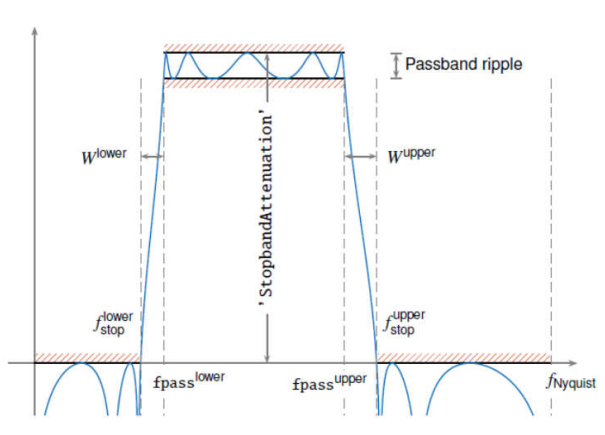
\includegraphics[scale=0.60]{Chapter1/bandPassFilter}
\caption{Band Pass Filter Frequency Response}
\label{bandPassFilter}
\end{center}
\end{figure}

\subsubsection{Band Stop Filters}
The Band Stop Filter, (BSF) is another variety of frequency selective circuit that
functions in just the other thanks to the Band Pass Filter we tend to checked out before.
The band stop filter, additionally referred to as a band reject filter, passes all
frequencies with the exception of these inside a such stop band that are greatly
attenuated.\\
Also, a bit like the band pass filter, the band filter may be a second-order (two-pole)
filter having 2 cut-off frequencies, normally referred to as the -3dB or half-power
points manufacturing a good stop band information measure between these 2 -3dB
points.\\
So for a wide-band band stop filter, the filters actual stop band lies between its lower
and higher -3dB points because it attenuates, or rejects any frequency between
these 2 cut-off frequencies. The frequency response curve of a perfect band stop filter
is so given as:
\begin{figure}[H]  %h=positioning
\begin{center}
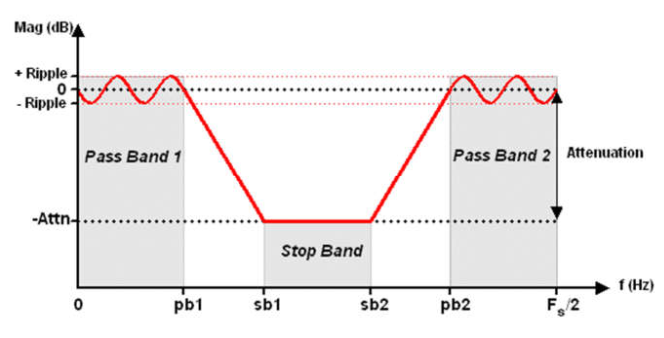
\includegraphics[scale=0.55]{Chapter1/stopBandFilter}
\caption{Band Stop Filter Frequency Response}
\label{stopBandFilter}
\end{center}
\end{figure}

\subsubsection{Low pass Filter}
A low-pass filter is a filter that permits signals under a cutoff frequency (known as the
pass band) and lessens signals over the cutoff frequency (known as the stop band). By
evacuating a few frequencies, the channel makes a smoothing impact. That is, the
channel delivers moderate changes in yield esteems to make it simpler to see patterns
and lift the general SNR with insignificant signal noise.

\begin{figure}[H]  %h=positioning
\begin{center}
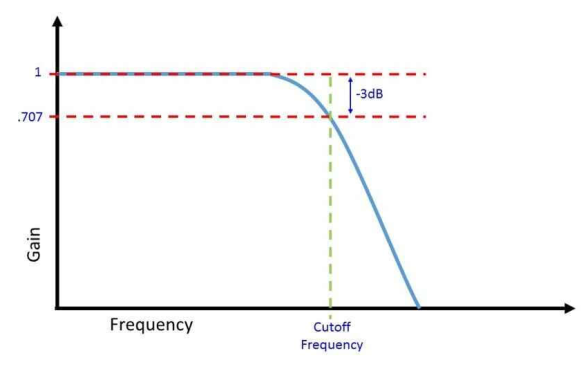
\includegraphics[scale=0.55]{Chapter1/lowPassFilter}
\caption{Low Pass Filter Frequency Response}
\label{lowPassFilter}
\end{center}
\end{figure}

%\section{Motivation}
%Motivated by the emergence of technological advancements and challenges in ...


%
%

%
%\section{UN Stainability Goals}

 %Goal 8 is shown which is Promote sustained, inclusive and sustainable economic growth, full and productive employment and decent work for all. As we will also discuss the economical long time benefits in next chapters. Our project will help industry in economic growth as well as it is providing a help to the meter readers.



%The conceptual frame work for the proposed method is comprises of three basic building blocks and detailed model is shown in Fig. \ref{fw}.
%\begin{enumerate}
%\item Network Formation Block.
%\item Neighbourhood Based Network Matrix Formation Block.
%\item Consensus Formation Block.
%\end{enumerate}
%
%In the network formation block, ...
%
%\FloatBarrier
%\begin{figure}[H]
%\begin{center}
%\hspace{15mm}
%\includegraphics[scale=0.35]{Chapter1/robocanesinternalstates}
%
%\protect\caption{Pseudo-code of Proposed Scheme for Cooperative Control of Networked Multi-Agent Systems.}
%\label{scode}
%\end{center}
%\end{figure}
%
%
\section{Report Break Down}
%
%This thesis deals with convergence analysis .... The main contributions of this work are summarized as follows:
%
%\begin{enumerate}
%\item  Initially a design ....
%
%\item An extended ....
%
%
%\item Modeled a ....
%
%\end{enumerate}
%
%The main contribution of this work is to propose a new way ....
%
%
%
%
%\section{Thesis Outline}
%
%
The major focus of this report is on the findings of the proposed project i.e. Speech Processing Using MATLAB

This Report is organized as follows:
\vspace{5mm}

In chapter 2, literature review is provided in detail about the work which is already been done on speech processing using MATLAB and will give a brief details about the articles, papers and literature review.
\vspace{5mm}


In Chapter 3, Proposed Methodology is presented in which you will be able to see the method we will work on the designing of a complete project source code to the diagrams.

\vspace{5mm}


In Chapter 4, Result and Simulations are being discussed, in which you will see all kind of finding related to the speech processing using MATLAB.


\vspace{5mm}

In Chapter 5, we have concluded and summarized the project work and also presented few new research ideas for future studies.


%\begin{equation}
%F=\sum_{n=0}^i(x_i(0)-x_j(0))^2
%%stackrel[u]{v}{T}=\stackrel[u]{v}{L}+\stackrel[u]{v}{L}\underset{W\epsilon V\cap w\neq u}{\sum}\stackrel[v]{w}{L}
%\end{equation}
